\documentclass[border=8pt]{standalone}
\usepackage{tikz}
\usetikzlibrary{arrows.meta, positioning, calc}

\begin{document}
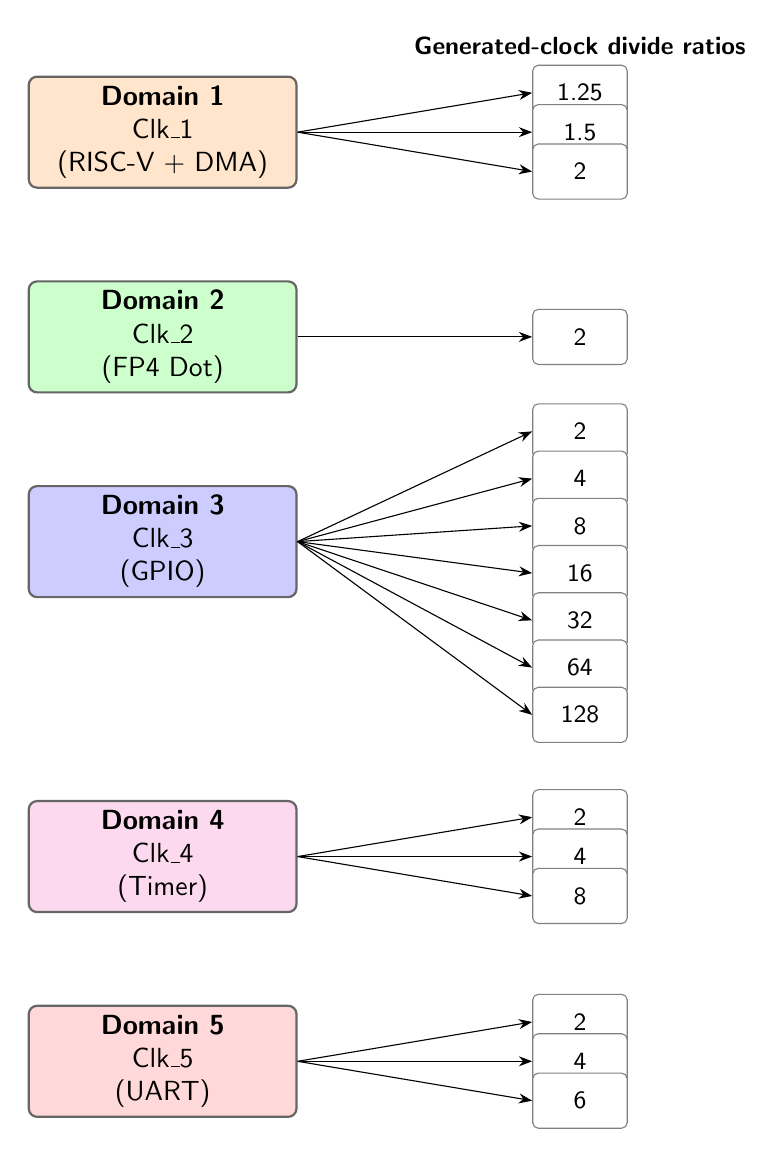
\begin{tikzpicture}[
  font=\sffamily,
  dbox/.style={rectangle, rounded corners=3pt, draw=black!60, thick, fill=#1,
               minimum height=10mm, minimum width=34mm, align=center},
  rbox/.style={rectangle, rounded corners=2pt, draw=black!50, thin, fill=white,
               minimum height=7mm, minimum width=12mm, align=center, font=\sffamily\small},
  lbl/.style={font=\sffamily\small},
  >=Stealth,
]

\node[lbl] at (5.3,1.1) {\textbf{Generated-clock divide ratios}};

% ---- Domain 1 (3 ratios) ----
\node[dbox=orange!20] (d1) at (0,0) {\textbf{Domain 1} \\ Clk\_1 \\ (RISC-V + DMA)};
\node[rbox] (d1r1) at (5.3,0.5)  {1.25};
\node[rbox] (d1r2) at (5.3,0)    {1.5};
\node[rbox] (d1r3) at (5.3,-0.5) {2};
\foreach \n in {d1r1,d1r2,d1r3}{ \draw[->] (d1.east) -- (\n.west); }

% ---- Domain 2 (1 ratio) ----
\node[dbox=green!20] (d2) at (0,-2.6) {\textbf{Domain 2} \\ Clk\_2 \\ (FP4 Dot)};
\node[rbox] (d2r1) at (5.3,-2.6) {2};
\draw[->] (d2.east) -- (d2r1.west);

% ---- Domain 3 (7 ratios) ----
\node[dbox=blue!20] (d3) at (0,-5.2) {\textbf{Domain 3} \\ Clk\_3 \\ (GPIO)};
\node[rbox] (d3r1) at (5.3,-3.8)  {2};
\node[rbox] (d3r2) at (5.3,-4.4)  {4};
\node[rbox] (d3r3) at (5.3,-5.0)  {8};
\node[rbox] (d3r4) at (5.3,-5.6)  {16};
\node[rbox] (d3r5) at (5.3,-6.2)  {32};
\node[rbox] (d3r6) at (5.3,-6.8)  {64};
\node[rbox] (d3r7) at (5.3,-7.4)  {128};
\foreach \n in {d3r1,d3r2,d3r3,d3r4,d3r5,d3r6,d3r7}{ \draw[->] (d3.east) -- (\n.west); }

% ---- Domain 4 (3 ratios) ----
\node[dbox=magenta!15] (d4) at (0,-9.2) {\textbf{Domain 4} \\ Clk\_4 \\ (Timer)};
\node[rbox] (d4r1) at (5.3,-8.7) {2};
\node[rbox] (d4r2) at (5.3,-9.2) {4};
\node[rbox] (d4r3) at (5.3,-9.7) {8};
\foreach \n in {d4r1,d4r2,d4r3}{ \draw[->] (d4.east) -- (\n.west); }

% ---- Domain 5 (3 ratios) ----
\node[dbox=red!15] (d5) at (0,-11.8) {\textbf{Domain 5} \\ Clk\_5 \\ (UART)};
\node[rbox] (d5r1) at (5.3,-11.3) {2};
\node[rbox] (d5r2) at (5.3,-11.8) {4};
\node[rbox] (d5r3) at (5.3,-12.3) {6};
\foreach \n in {d5r1,d5r2,d5r3}{ \draw[->] (d5.east) -- (\n.west); }

\end{tikzpicture}
\end{document}
